\documentclass[a4paper]{article}
\usepackage{graphicx}
\usepackage{amsfonts}
\usepackage[ruled,vlined]{algorithm2e}
\usepackage[a4paper, total={6in, 10in}]{geometry}
\graphicspath{ {./images/} }
\title{Unsupervised Data Augmentation Experiments}
\author{Michael Morris}

\begin{document}
\maketitle
\section{Semi Supervised Learning}
Semi supervised learning is a method of training machine learning models which leverages unlabelled data. This reduces the labelling cost of an expert labeller and means that datasets with large amounts of unlabelled data can be used. Historically this has been done by generating a decision boundary based on the positions of unlabelled data in relation to labelled data. 

\begin{figure}[h]
  \begin{center}
    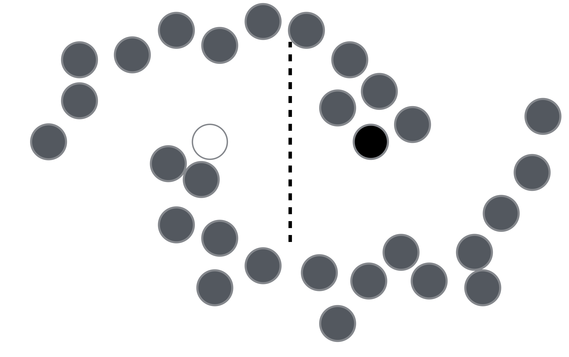
\includegraphics[width=.4\textwidth]{SSL}
    \caption{Decision boundary with unsupervised examples}
  \end{center}
\end{figure}
The unlabelled datapoints can be categorised correctly by their spatial relation to the two labelled samples. The methods to do this are based on the following assumptions:
\begin{itemize}
  \item Points which are close together are likely to be in the same class 
  \item The data tends to form distinct clusters
  \item The data can be expressed in fewer dimensions than its inputs.
\end{itemize}
These lead to pseudo labelling where the model is updated as if these labels are correct. 

\section{Unsupervised Data Augmentation}
Unsupervised Data Augmentation (UDA) is a method of leveraging unlabelled data based on state of the art data augmentation policies. In UDA unlabelled data is augmented: $\hat{x}=q(x,\epsilon)$ and the divergence in outputs between the original and augmented data is minimised for consistency training. This follows the assumption that the original and augmented samples have the same class, and by learning distinguishing features the distance between the labelled and unlabelled data will be minimised. The loss function for the labelled data is categorical cross entropy. For the unlabelled data is the Kullback-Leibler divergence between the original and augmented data. The unsupervised loss is weighted by a variable $\lambda$ giving the full objective function where $U$ and $L$ represent unlabelled and labelled data respectively:
\begin{equation}
\min_{\theta} \mathcal{J}(\theta) =\mathbb{E}_{x,y^* \in L}[-\log p_\theta (y^* | x)]+\lambda\mathbb{E}_{x \in U}\mathbb{E}_{\hat{x}\sim q(\hat{x} \mid x)}[\mathcal{D}_{KL}(p_{\tilde{\theta}}(y \mid x) \parallel p_\theta (y \mid \hat{x})) ]
\end{equation}
Where the KL divergence is:
\begin{equation}
\mathcal{D}_{KL}(P \parallel Q) = \sum_{x \in X} P_{(x)} \log \left(\frac{P_{(x)}}{Q_{(x)}}\right)
\end{equation}
The training objective is illustrated below:
\begin{figure}[h]
  \begin{center}
    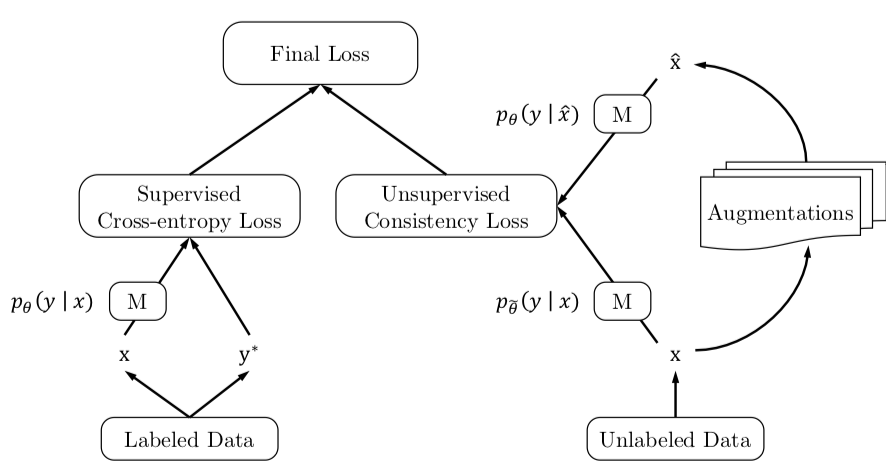
\includegraphics[width=.8\textwidth]{training_objective}
    \caption{Training objective for UDA}
  \end{center}
\end{figure}


The pseudo code is as follows:
\begin{algorithm}[htbp]
\SetAlgoLined
duplicate data so equal number of potential batches in labelled and unlabelled sets\;
shuffle data\;
 split into batches\;
 \For{epochs}{
 	\For{batches}{
		\If{labelled batch}{
			calculate $p_\theta (y^* | x)$\;
   			$Lloss = \mathbb{E}_{x,y^* \in L}[-\log p_\theta (y^* | x)]$\;
		}
		\If {unlabelled batch}{
			create $\hat{x}$ by augmenting $x$\;
			$Uloss = \lambda\mathbb{E}_{x \in U}\mathbb{E}_{\hat{x}\sim q(\hat{x} \mid x)}[\mathcal{D}_{KL}(p_{\tilde{\theta}}(y \mid x) 	\parallel p_\theta (y \mid \hat{x})) ]$\;
		}
		minimise $Uloss+Lloss$\;
 	}
	calculate accuracy from labelled validation set\;
 }
\caption{UDA Algorithm}
\end{algorithm}



\end{document}